\section{Empirical Results and Multi-Biome Dynamics}
\label{sec:results}

\subsection{Two-Way Variance Decomposition Across All Seven Metropolises}
To evaluate how dynamic atmospheric fluctuations interact with stationary urban morphology, we partition the total sample variance ($\sigma^2$) of composite stress into temporal seasonality (between-month), spatial urban morphology (between-hex), and residual spatio-temporal coupling across all seven metropolitan regions:
\begin{equation}
    \sigma^2_{\text{total}} = \sigma^2_{\text{temporal (between-month)}} + \sigma^2_{\text{spatial (between-hex)}} + \sigma^2_{\text{residual (spatio-temporal)}}
\end{equation}

The empirical variance shares demonstrate how biophysical regime dictates risk structure across India:
\begin{itemize}
    \item \textbf{High-Seasonality Continental Regimes (Bikaner \& Delhi):} Bikaner exhibits $98.0\%$ temporal variance ($4.1\%$ spatial), while Delhi displays $86.1\%$ temporal variance ($14.2\%$ spatial). In these northern continental biomes, severe annual meteorological swings (hyper-arid summer heatwaves followed by winter inversions) dominate overall stress levels.
    \item \textbf{Plateau and Deltaic Metropolises (Mumbai, Indore, Kolkata, \& Hyderabad):} Exhibit balanced dynamics with $72.7\%\text{--}78.6\%$ temporal variance and $20.0\%\text{--}27.4\%$ spatial variance. Urban morphology (built density, transportation corridors, and local vegetative cover) plays a substantial role in differentiating micro-neighborhood exposure.
    \item \textbf{Inland Rainshadow Regime (Coimbatore):} Coimbatore exhibits the highest spatial share in India ($42.8\%$ spatial, $53.9\%$ temporal, $3.4\%$ residual). In the absence of massive extreme weather swings, micro-spatial urban form (building density and local tree canopy) dictates vulnerability.
\end{itemize}

\begin{figure}[t]
    \centering
    \IfFileExists{figures/Figure3_variance_decomposition.png}{%
        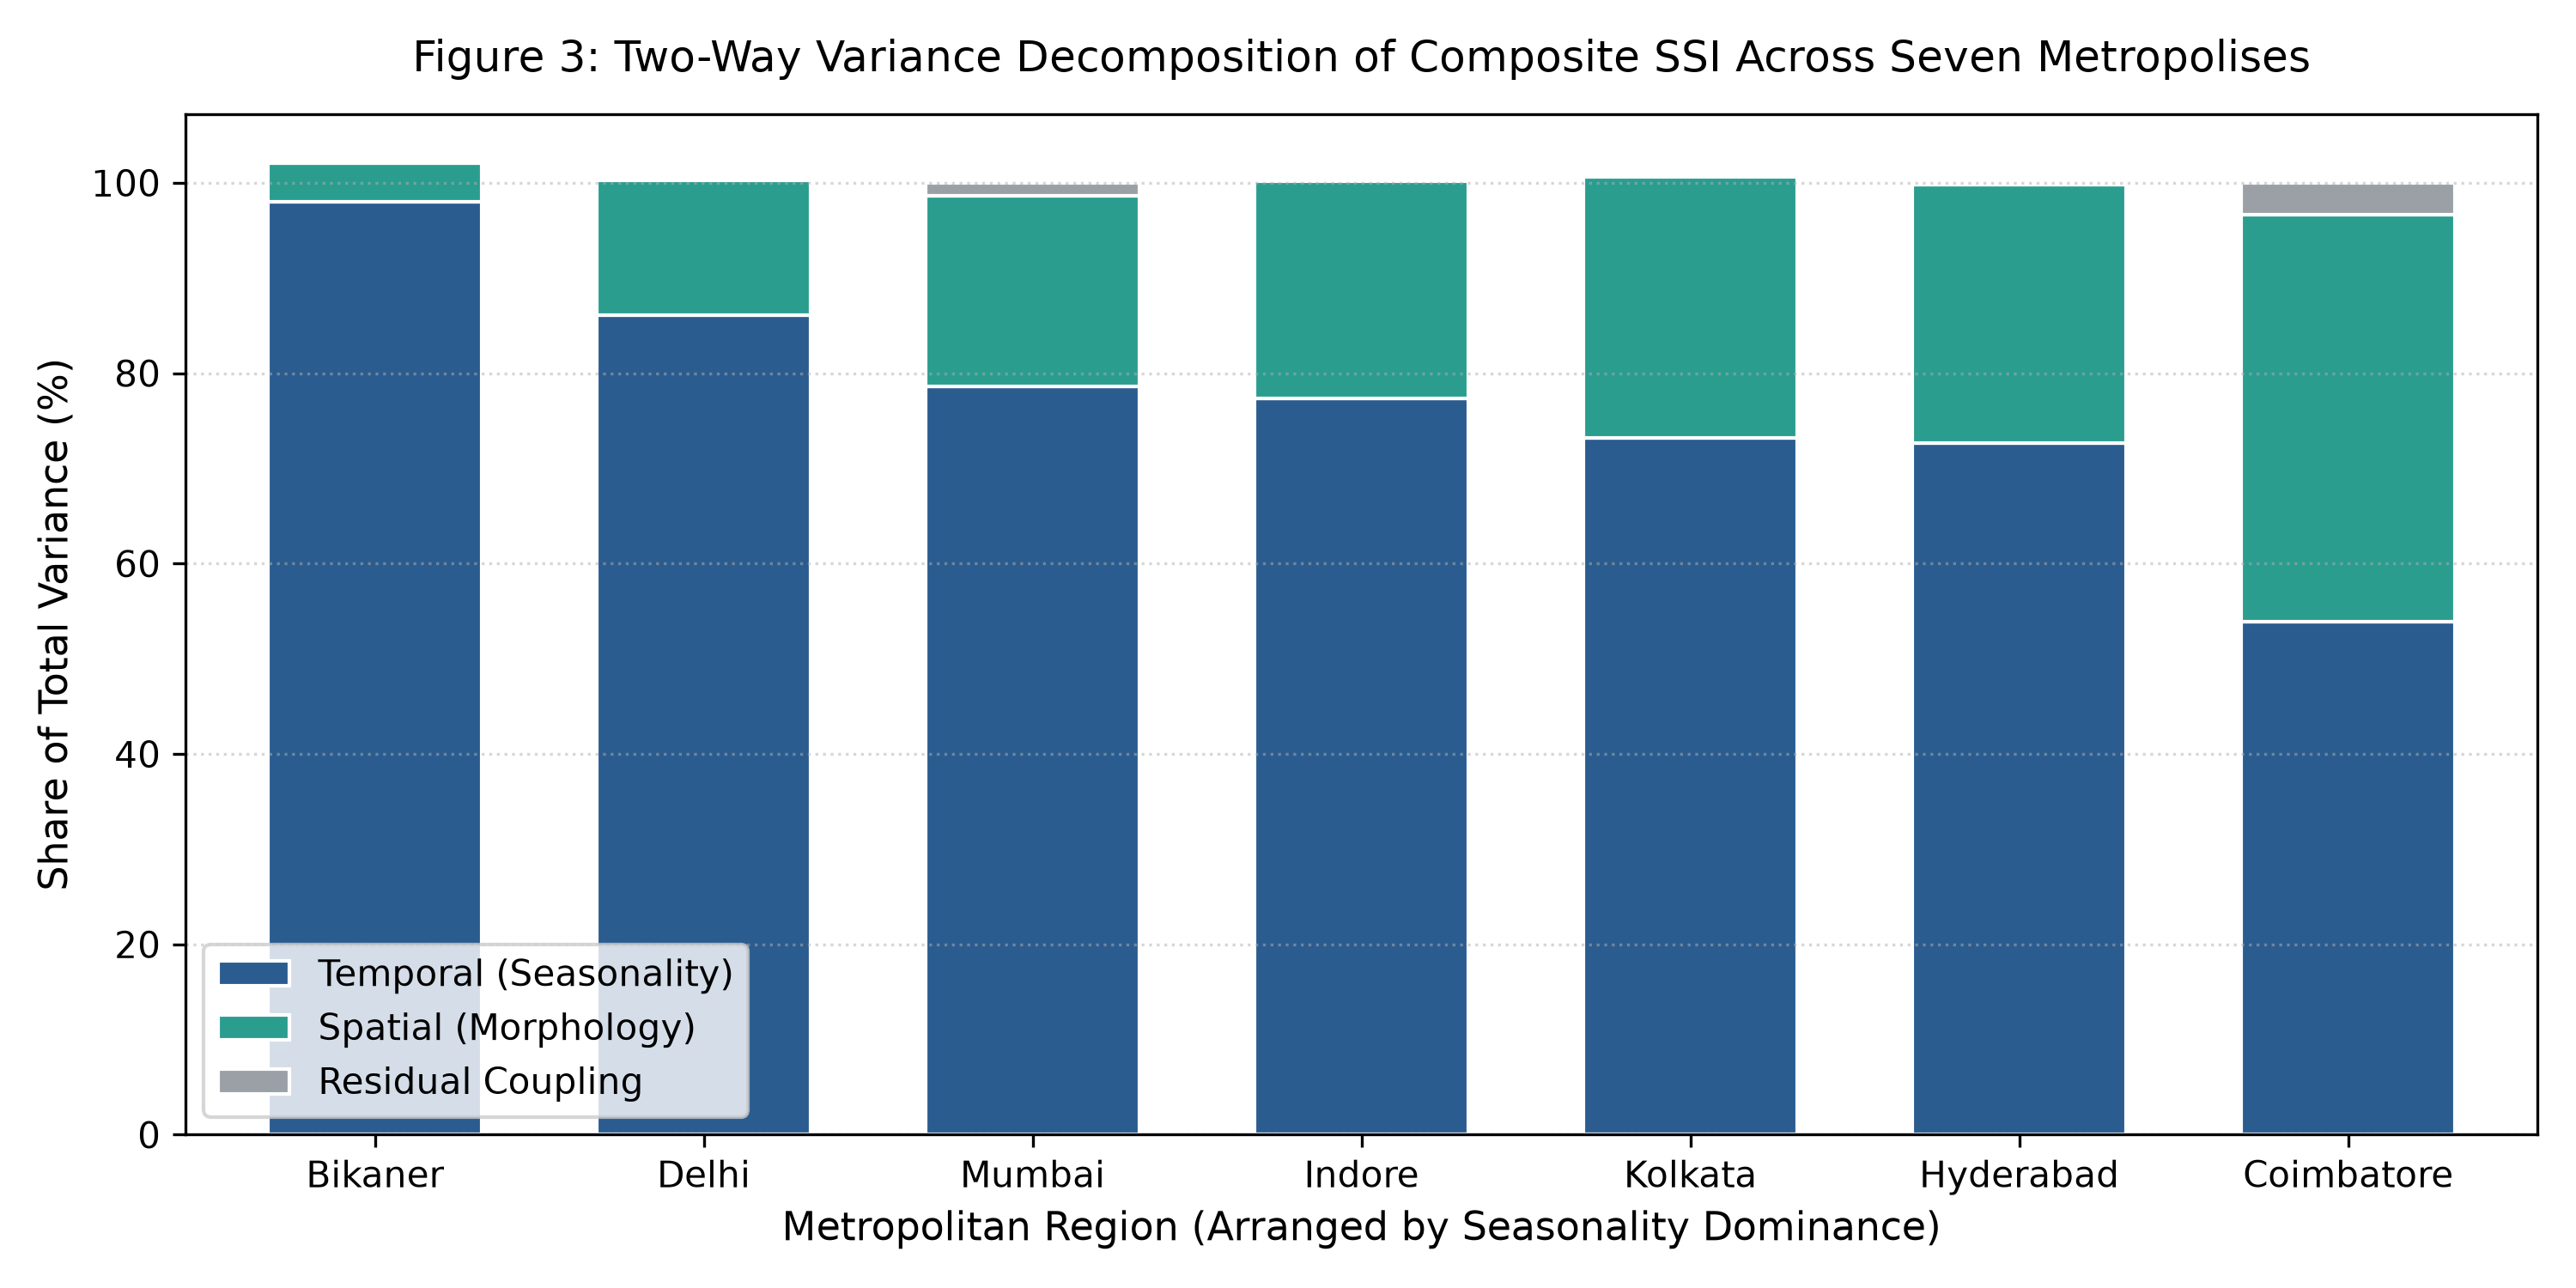
\includegraphics[width=0.95\textwidth]{figures/Figure3_variance_decomposition.png}%
    }{%
        \vspace{1em}
        \fbox{\parbox{0.95\textwidth}{\centering\small\textbf{[Figure 3: Two-Way Variance Decomposition Across Seven Metropolises]}\\
        \textit{Generated via \texttt{colab\_analysis.py} from \texttt{final\_7\_cities.parquet} ($N = 334,332$). Compares temporal seasonality shares vs. spatial morphological shares across the seven biomes.}}}%
        \vspace{1em}
    }
    \caption{Two-way variance decomposition of composite SSI across all seven metropolitan study regions. Metropolises are arranged along the gradient of temporal seasonality dominance, contrasting continental regimes (Bikaner, Delhi) with spatial morphology-driven regimes (Coimbatore, Mumbai, Kolkata).}
    \label{fig:variance_decomposition}
\end{figure}

\subsection{Cross-Biome Discriminant Validity}
Across the 334,332 empirical panel observations, composite SSI values exhibit highly significant differentiation across the seven climatic biomes (One-Way ANOVA $F = 6,888, p < 10^{-15}$; non-parametric Kruskal-Wallis $H = 30,024, p < 10^{-15}$).

As detailed in Table~\ref{tab:city_biomes}, mean SSI levels and hazard signatures align with geographical expectations:
\begin{itemize}
    \item \textbf{Kolkata (Mean SSI = 0.5748):} Demonstrates the highest cumulative stress in India, driven by the intense co-occurrence of high wet-bulb sultriness, dense deltaic urban core built fraction, and severe winter particulate stagnation. Over $67.6\%$ of Kolkata hex-months fall within the \textit{Extreme} risk band ($\Omega_{\text{compound}} = 25.06\%$).
    \item \textbf{Delhi (Mean SSI = 0.5592):} Characterized by extreme annual thermal spreads (summer heat index $>40^\circ\text{C}$ vs. winter $<13^\circ\text{C}$) compounded by massive winter aerosol saturation ($\text{PM}_{2.5}$ mean $257.3\ \mu\text{g}/\text{m}^3$), resulting in $56.9\%$ of hex-months in the \textit{Extreme} band ($\Omega_{\text{compound}} = 30.91\%$).
    \item \textbf{Bikaner (Mean SSI = 0.5081):} Displays chronic, severe year-round water scarcity (mean water deficit $236.1\text{ mm}/\text{month}$, peaking at $639.8\text{ mm}$) and high vegetative degradation ($0.7879$). Joint-tail compound activation reaches $40.44\%$, with $50.63\%$ in the \textit{Extreme} band.
    \item \textbf{Mumbai (Mean SSI = 0.4884):} Displays moderate-to-high baseline maritime sultriness with acute summer water deficits ($0.87$) that experience sharp relief during the southwest monsoon deluge ($0.34$ in August; seasonal spread $+0.53$). Compound trigger occurs in $14.43\%$ of observations ($45.03\%$ \textit{Extreme}).
    \item \textbf{Hyderabad (0.4113), Indore (0.3813), and Coimbatore (0.3326):} Exhibit significantly lower baseline stress. Coimbatore represents India's least stressed study metropolis, benefiting from lower aerosol concentrations (mean $62.2\ \mu\text{g}/\text{m}^3$) and lower compound activation frequencies ($0.68\%$).
\end{itemize}

\subsection{Impact of Smooth Asymptotic Compound Coupling}
Comparing linear weighted composites against the non-linear formulation (Equation~\ref{eq:smooth_ssi}) confirms that bivariate joint-tail compounding introduces a significant, non-substitutable escalation during multi-hazard shocks.

At moderate stress levels (deciles D1--D5), linear and compound scores display near-perfect agreement ($r = 0.933$, rank correlation $\rho = 0.942$). However, across the top 10th percentile (extreme compound events where both heat and pollution simultaneously breach their 90th percentiles), the non-linear interaction term introduces a \textbf{+25.3\% average stress escalation (+0.162 absolute index increase)}.

Crucially, the smooth asymptotic damping term $(1.0 - \text{SSI}_{\text{lin}})$ guarantees that \textbf{0.00\% of observations hit an artificial ceiling of 1.0000} (maximum observed $\text{SSI} = 0.9807$). In contrast, standard additive models clamp over $20\%$ of multi-city panel records at an artificial ceiling of $1.0000$, destroying intra-extreme spatial discrimination.

\subsection{Pan-India Urban Stress Archetypes}
Unsupervised $k$-means clustering across the 334,332 observations reveals six distinct, stable pan-India stress archetypes (Silhouette coefficient $s = 0.147 > 0$; bootstrap Adjusted Rand Index $\text{ARI} = 0.812 \pm 0.034$, confirming robust cluster stability) (Table~\ref{tab:archetype_profiles} and Figure~\ref{fig:archetype_radar}):

\begin{table}[t]
\centering
\small
\caption{Pan-India urban sustainability stress archetypes ($k = 6$) derived from unsupervised clustering across 334,332 hexagonal panel records.}
\label{tab:archetype_profiles}
\begin{tabularx}{\textwidth}{@{}c r r r r r X@{}}
\toprule
\textbf{Archetype} & \textbf{Heat} & \textbf{Water} & \textbf{Veg} & \textbf{Pollution} & \textbf{Exposure} & \textbf{Dominant Environmental Typology} \\
\midrule
1 & 0.189 & 0.240 & 0.500 & 0.208 & 0.146 & Suburban Peripheral / Baseline Low Stress \\
2 & 0.819 & 0.901 & 0.616 & 0.466 & 0.113 & Severe Arid Heat \& Chronic Water Deficit \\
3 & 0.209 & 0.268 & 0.678 & 0.213 & 0.726 & High Built Exposure \& Vegetative Depletion \\
4 & 0.094 & 0.168 & 0.383 & 0.972 & 0.112 & Acute Winter Atmospheric Inversion \& Smog \\
5 & 0.072 & 0.145 & 0.726 & 0.979 & 0.515 & Dense Urban Corridor / High Smog Saturation \\
6 & 0.813 & 0.874 & 0.712 & 0.451 & 0.671 & Compound Multi-Hazard Core Hotspot \\
\bottomrule
\end{tabularx}
\end{table}


\begin{figure}[t]
    \centering
    \IfFileExists{figures/Figure7_archetype_radar.png}{%
        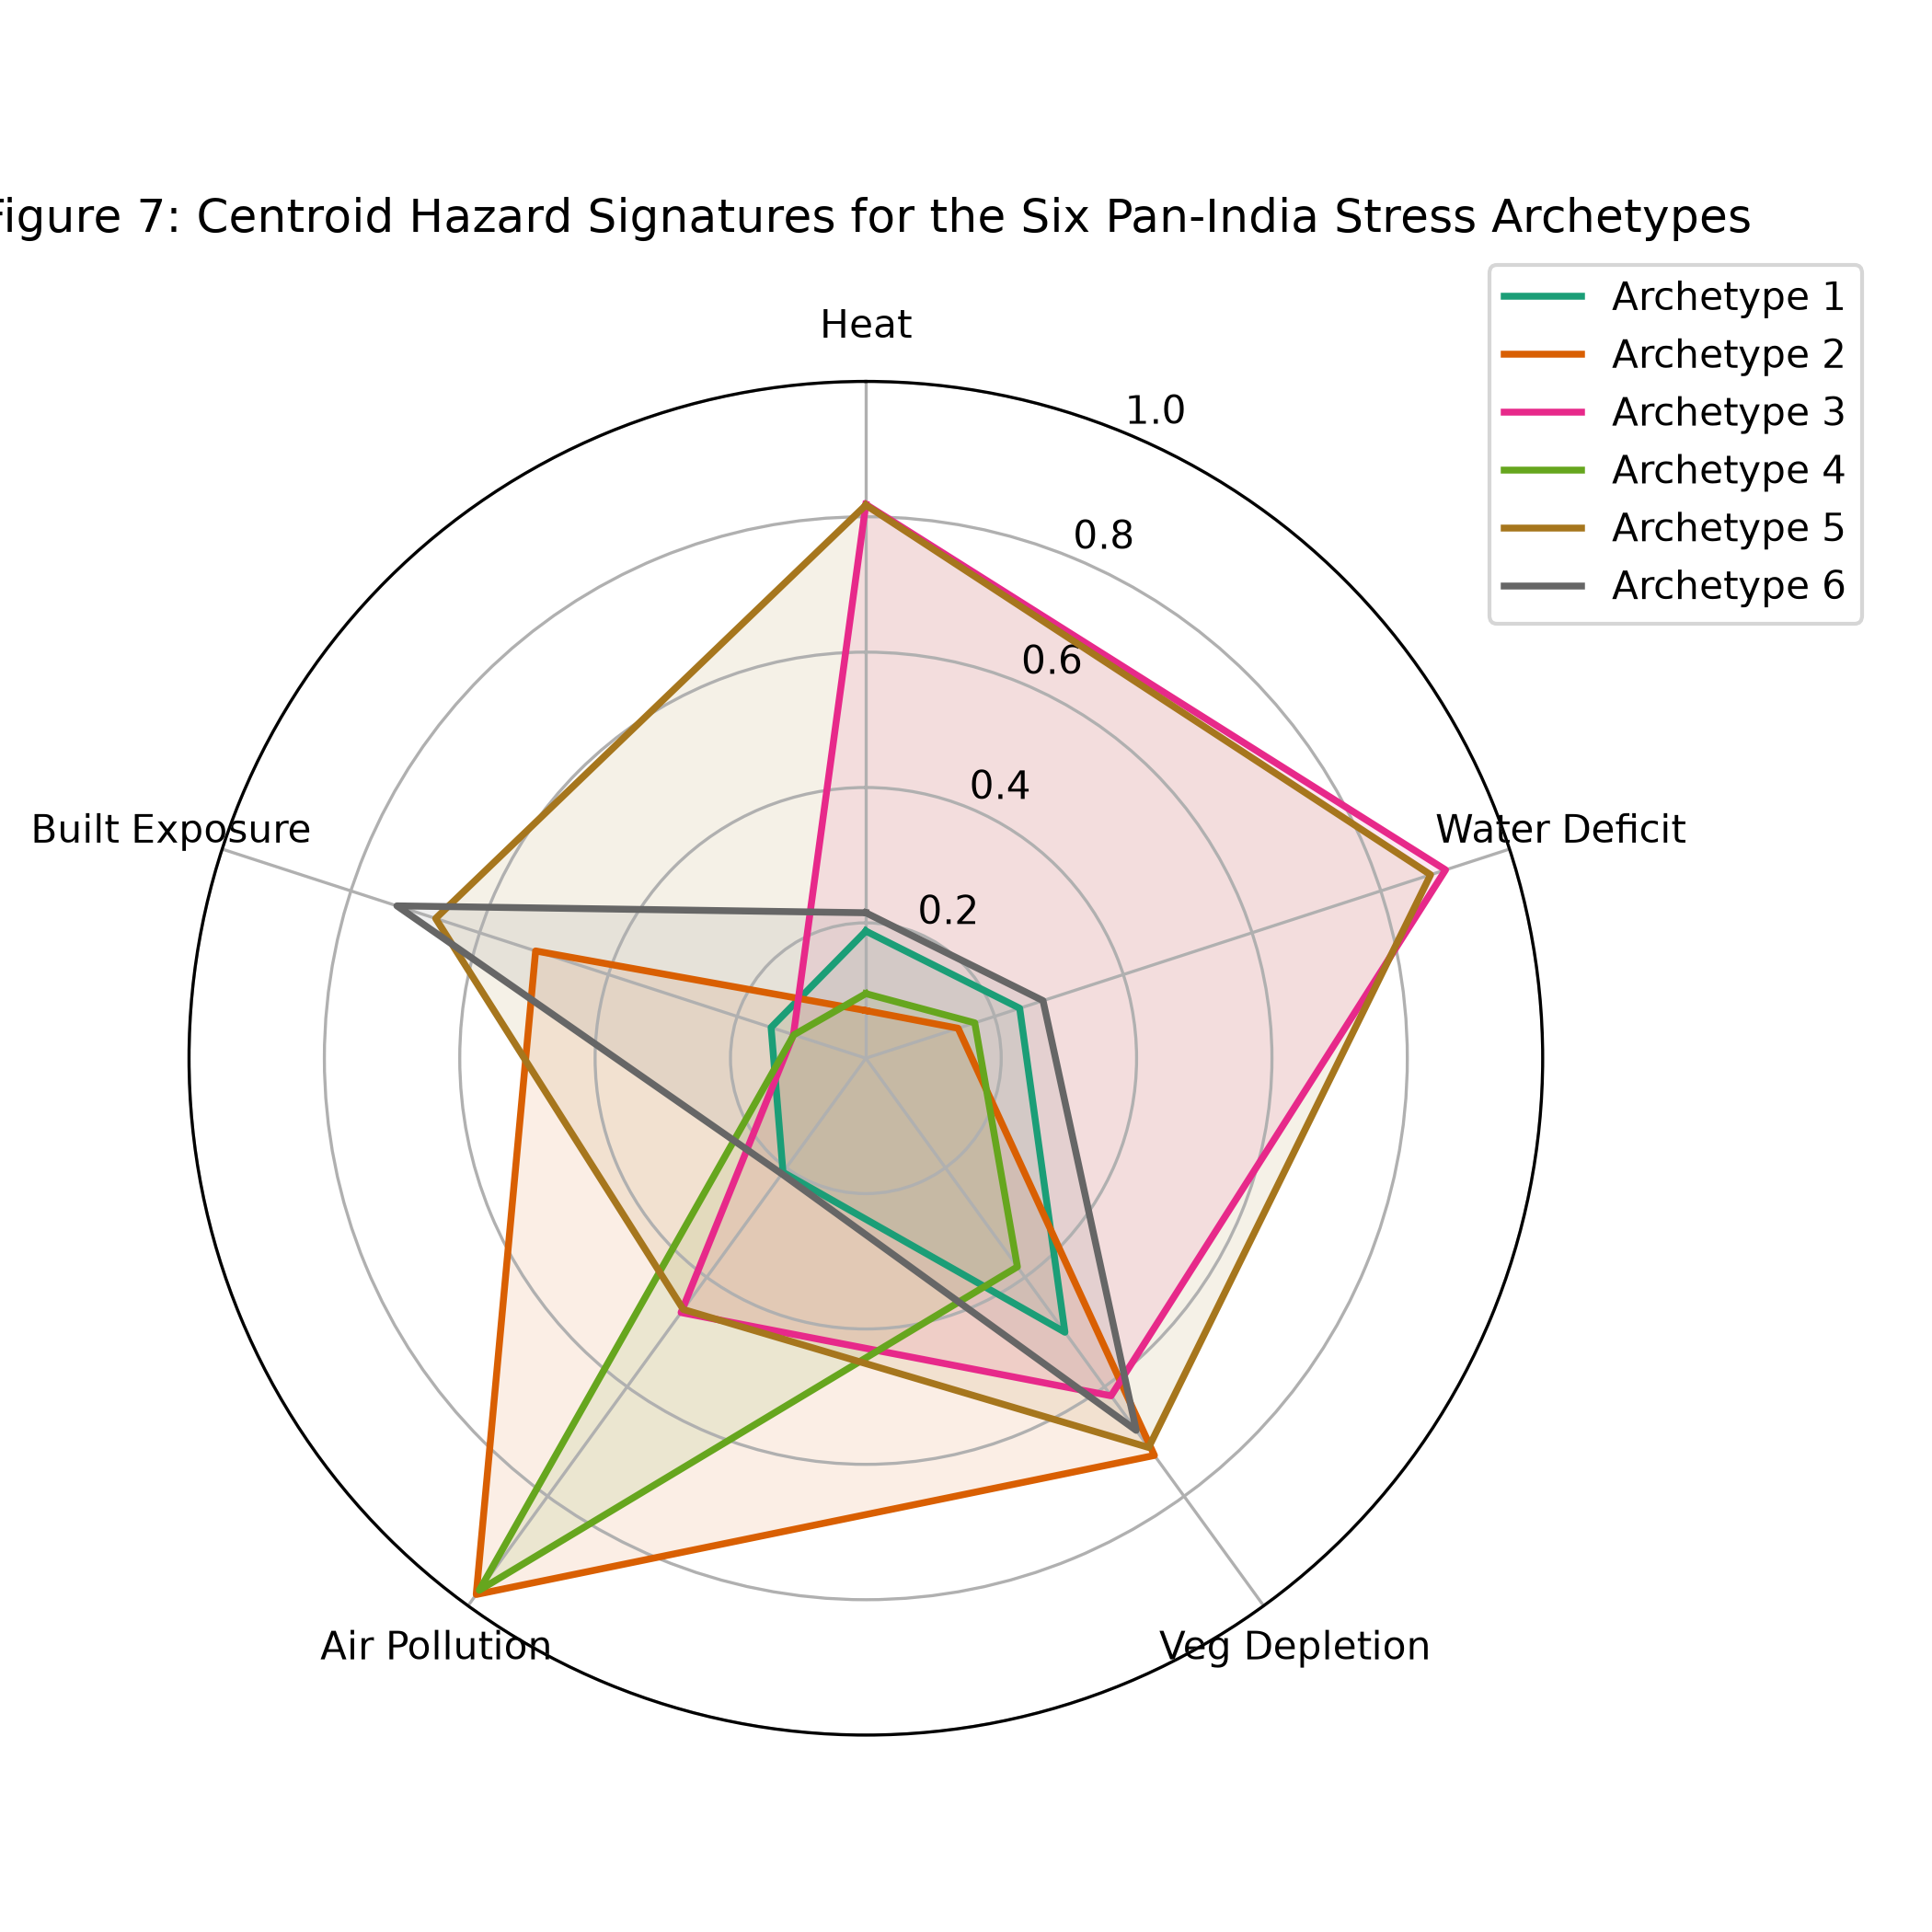
\includegraphics[width=0.75\textwidth]{figures/Figure7_archetype_radar.png}%
    }{%
        \vspace{1em}
        \fbox{\parbox{0.75\textwidth}{\centering\small\textbf{[Figure 7: Archetype Hazard Signatures Radar Chart]}\\
        \textit{Generated via \texttt{colab\_analysis.py} from \texttt{final\_7\_cities.parquet} ($N = 334,332$). Visualizes 5-dimensional hazard centroid profiles for each of the six pan-India urban stress archetypes.}}}%
        \vspace{1em}
    }
    \caption{Hazard centroid radar profiles for the six pan-India urban stress archetypes ($k = 6$) derived from the pooled 334,332-record panel. Distinct directional signatures highlight the necessity of typology-specific municipal adaptation strategies.}
    \label{fig:archetype_radar}
\end{figure}

\begin{itemize}
    \item \textbf{Archetype 1 (Peripheral Baseline -- 21.3\% prevalence):} Low scores across all five hazards ($\text{SSI} \approx 0.25$). Dominates suburban and peri-urban agricultural buffers.
    \item \textbf{Archetype 2 (Arid Thermal-Hydrological Stress -- 26.6\% prevalence):} High heat ($0.819$) and extreme water deficit ($0.901$) with low built density ($0.113$). Encompasses dry-season Bikaner, rural Delhi fringes, and pre-monsoon Deccan plateaus.
    \item \textbf{Archetype 3 (Congested Urban Core -- 11.6\% prevalence):} High built exposure ($0.726$) and vegetative canopy depletion ($0.678$) under moderate atmospheric background stress. Marks densely built commercial and residential cores.
    \item \textbf{Archetype 4 (Atmospheric Smog Inversion -- 13.2\% prevalence):} Near-maximum particulate air pollution ($0.972$) occurring during winter thermal inversions in low-density or peripheral sectors.
    \item \textbf{Archetype 5 (High-Exposure Smog Corridor -- 13.1\% prevalence):} Severe concurrent air pollution ($0.979$) concentrated in densely built urban transport corridors ($0.515$).
    \item \textbf{Archetype 6 (Compound Multi-Hazard Core -- 14.2\% prevalence):} Acute convergence of extreme heat ($0.813$), severe water deficit ($0.874$), high built density ($0.671$), and canopy loss ($0.712$). Represents the highest-priority target for integrated urban resilience planning.
\end{itemize}
